\section{Simulation analysis}
\label{sec:simulation}

In this section we will be describing the simulations that we made on NGSpice where we made 4 scripts describing the given circuit (figure 1), as it is requested in T2's lab questions. After running the scripts, we will be able to compare the results we got from the theoretical analysis. \par
This simulation analysis includes 5 questions, from which the last two are answered using the same script (the circuit is the same, we only want different results).

\subsection{Question 1: }
For the first question of this simulation analysis we begun by adding the values for all the components used in the circuit, thus describing the circuit in order to simulate it. \par
All the simulation was done using the same node nomenclature as in figure 1. \par
After describing the circuit in a NGSpice script we simulated the operating point for $t<0$, for which $v_s=V_s$, in order to obtain the volatges in all nodes and the currents in all branches.\par
The results we got are in the table below:
\begin{table}[H]
  \centering
  \begin{tabular}{|l|r|}
    \hline    
    {\bf Name} & {\bf Value [A or V]} \\ \hline
    @c0[i] & 0.000000e+00\\ \hline
@g0[i] & -3.00677e-04\\ \hline
@r1[i] & 2.870701e-04\\ \hline
@r2[i] & -3.00677e-04\\ \hline
@r3[i] & -1.36064e-05\\ \hline
@r4[i] & 1.190255e-03\\ \hline
@r5[i] & -3.00677e-04\\ \hline
@r6[i] & 9.031846e-04\\ \hline
@r7[i] & 9.031846e-04\\ \hline
n1 & 5.025226e+00\\ \hline
n2 & 4.724476e+00\\ \hline
n3 & 4.104661e+00\\ \hline
n5 & 4.765766e+00\\ \hline
n6 & 5.702373e+00\\ \hline
n7 & -1.84781e+00\\ \hline
n8 & -2.79065e+00\\ \hline
n9 & -2.79065e+00\\ \hline

  \end{tabular}
  \label{tab:op1}
\end{table}

\subsection{Question 2: }
After completing the first step of the simulation analysis, we replaced the capacitor with a voltage source $V_x$ whose voltage is equal to $v_6-v_8$ as obtained in question 1, and did the same operating point simulation in order to obtain the voltages and currents in the circuit. \par
The reason we have to do this step is in all ways similar to the reason in question 2 of the theoretical analysis and is described in section 2.2. \par
The results we got from the simulation are in the table below:
\begin{table}[H]
  \centering
  \begin{tabular}{|l|r|}
    \hline    
    {\bf Name} & {\bf Value [A or V]} \\ \hline
    \input{op2_tab}
  \end{tabular}
  \label{tab:op2}
\end{table}

\subsection{Question 3: }
After getting the results from question 2 we then proceeded to make another NGSpice script simulating the natural response of the circuit (with no voltage sources connected), using the boundary conditions $v_6$ and $v_8$ as obtained in question 2. \par
In this question we made a transient analysis in order to get $v_6$ during the [0,20] $ms$ time window. This is, the variation of the voltage in node 6 as the capacitr discharges. \par
The result we got is in the plot below:
\begin{figure}[H] \centering
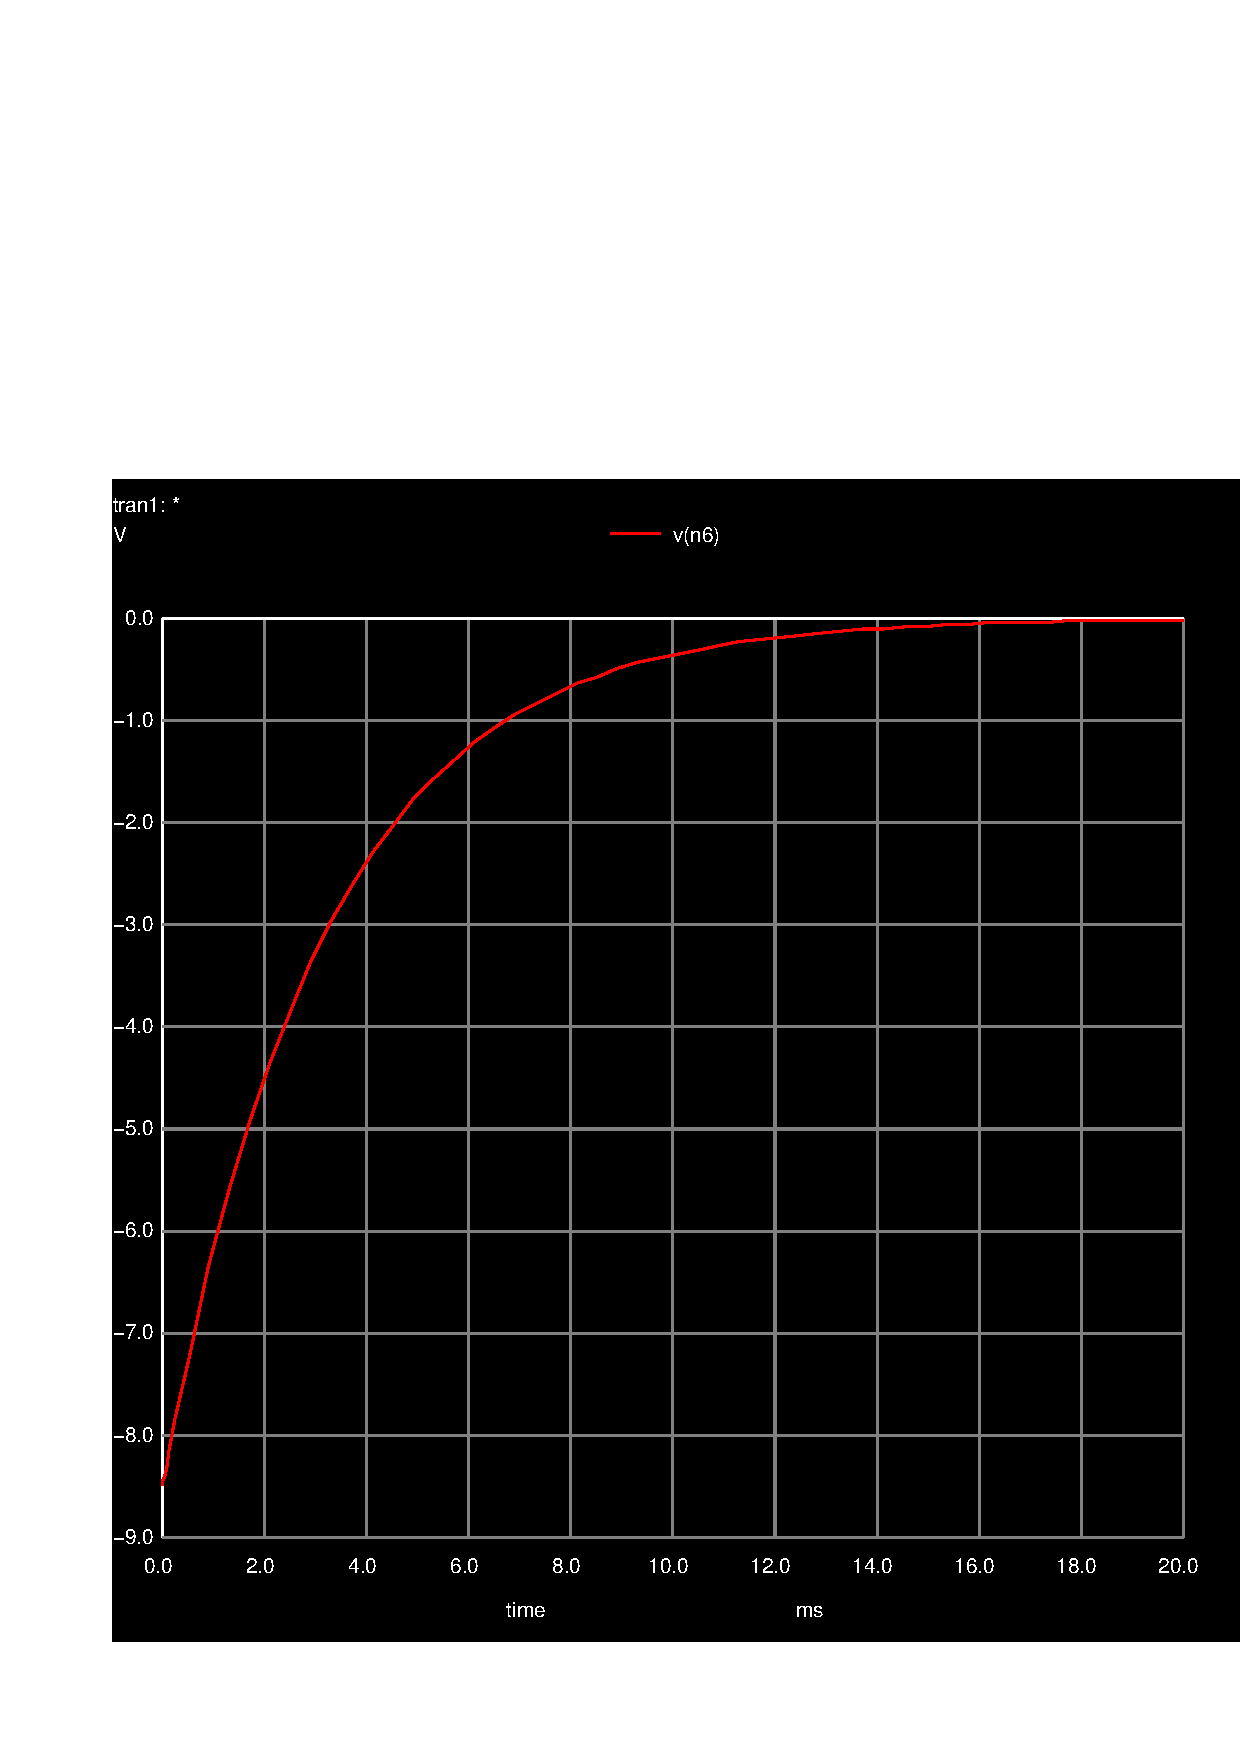
\includegraphics[width=0.7\linewidth]{../sim/transient3.pdf}
\caption{Transient Analysis of Question 3.}
\label{fig:transient3}
\end{figure}

\subsection{Question 4: }
This question and the next were answered using the same script as it features the same exact circuit. \par
In these two questions, we are simulating the circuit with $v_s(t)$ as given in figure 1.\par
In the present question 4, we will be simulating the total response (forced and natural together) on node 6 using a frequency of 1$kHz$ on the voltage source $v_s$, and the same time interval as in question 3. \par
The results we got are in the plots below, with the first one being the stimulus and the second one the response:
\begin{figure}[H] \centering
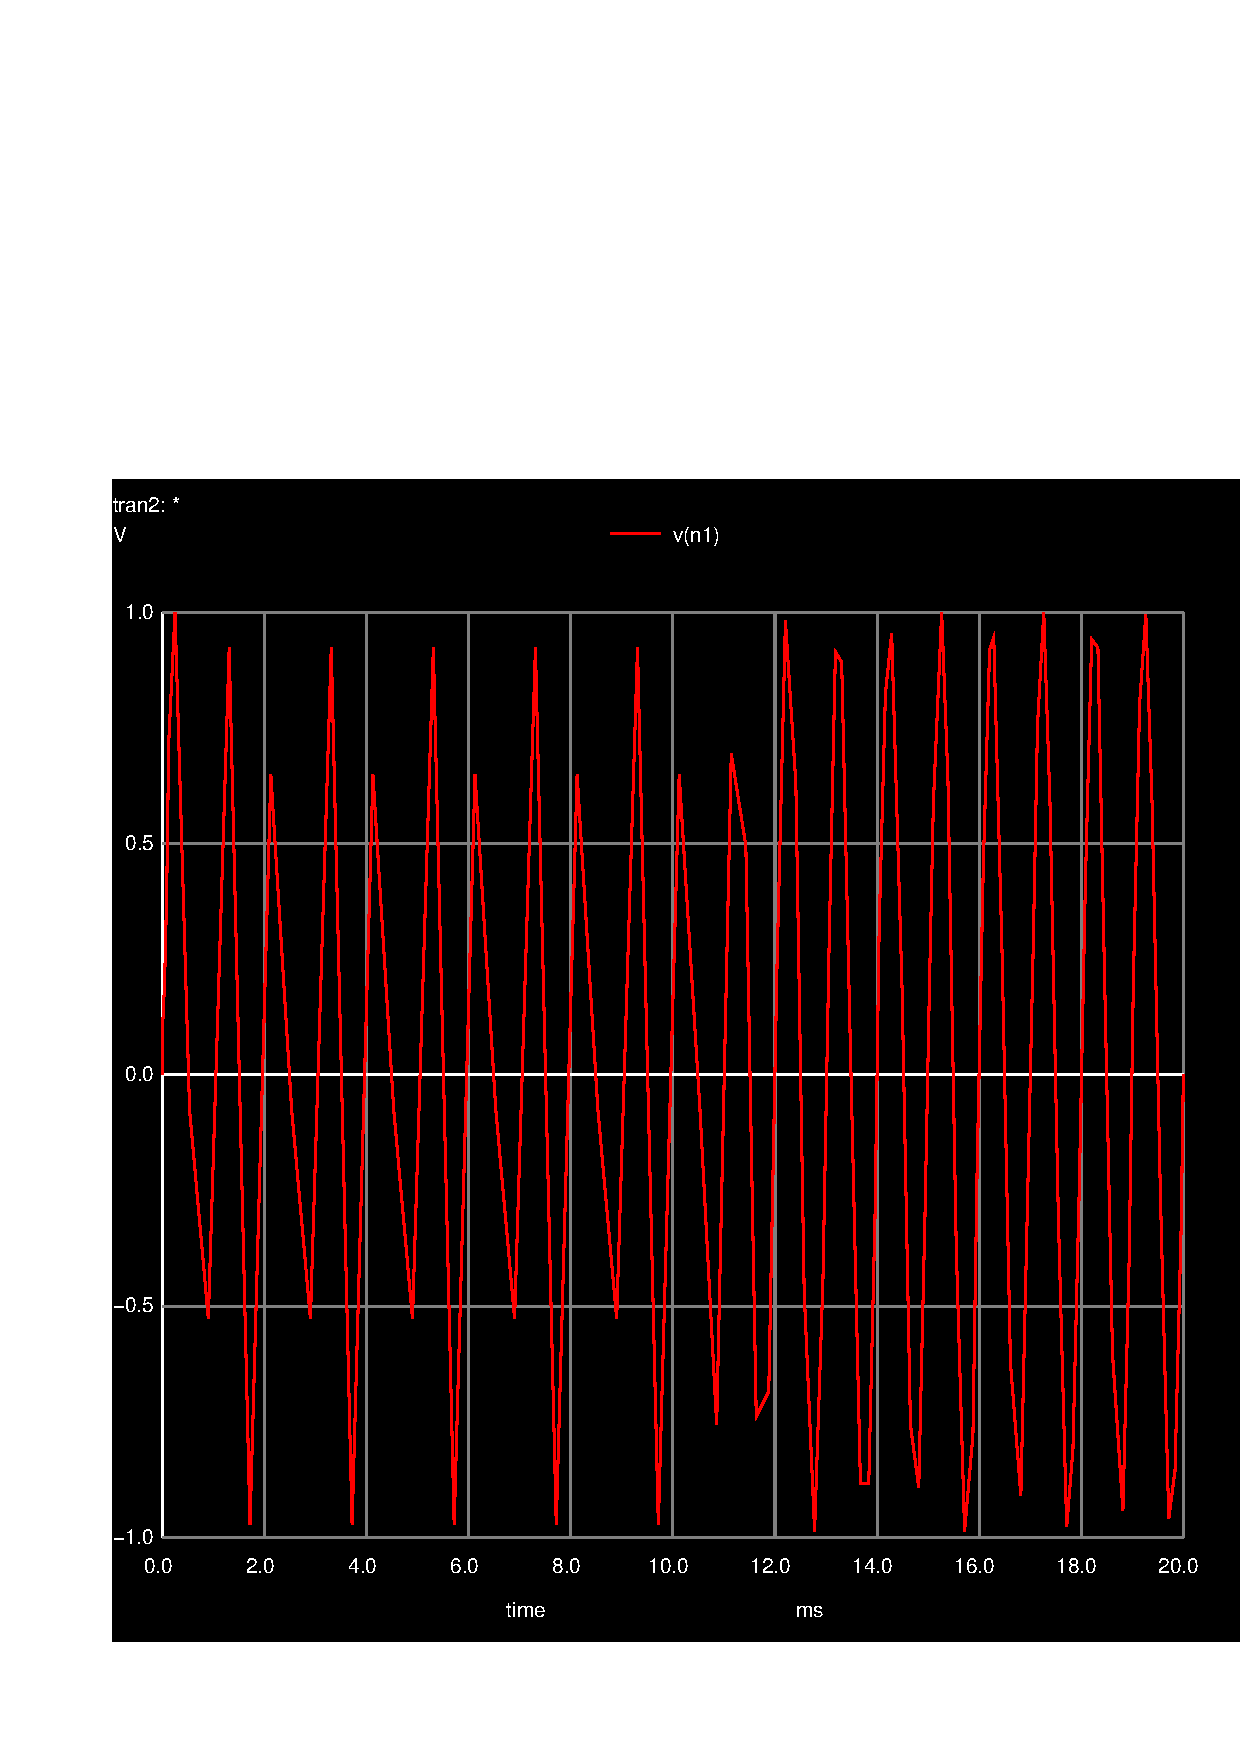
\includegraphics[width=0.7\linewidth]{../sim/transient4s.pdf}
\caption{Transient Analysis of the Stimulus on Question 4.}
\label{fig:transient4s}
\end{figure}

\begin{figure}[H] \centering
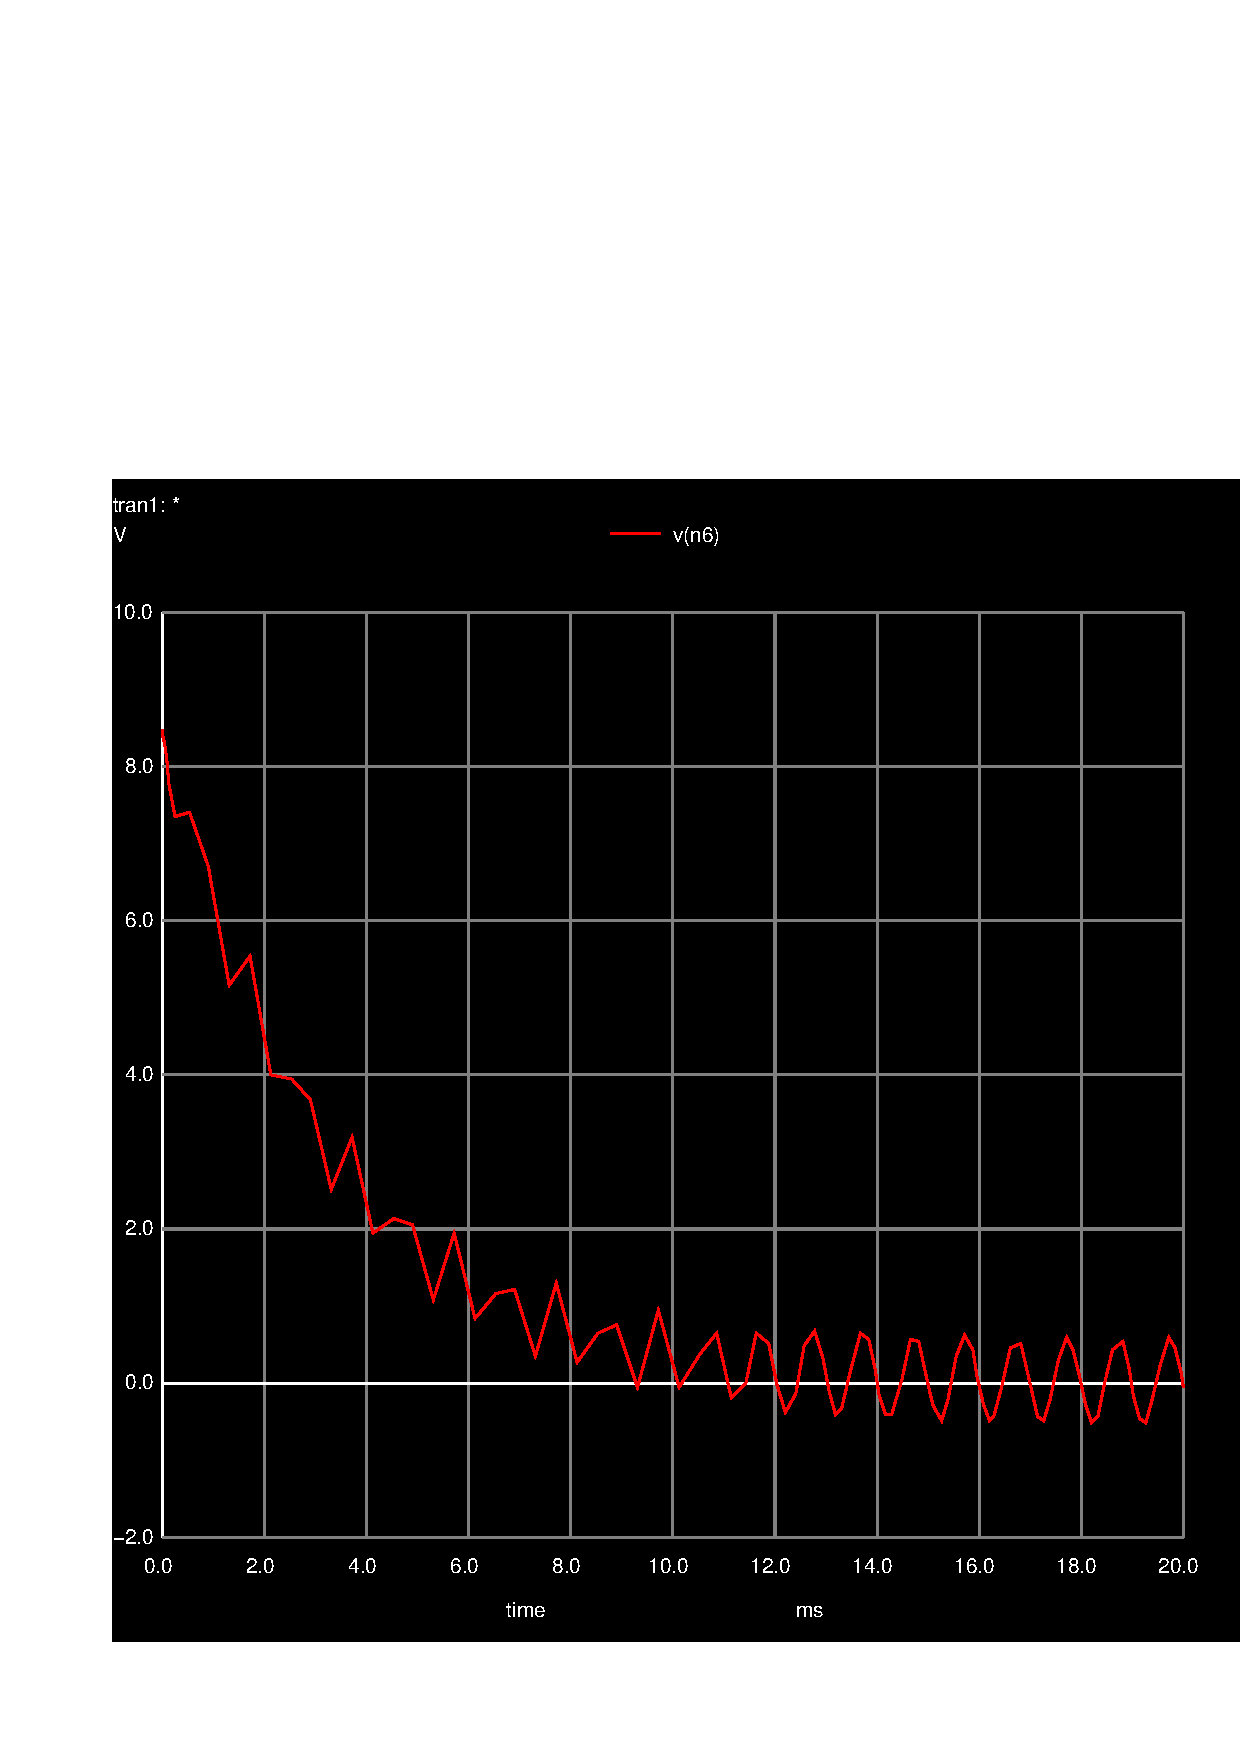
\includegraphics[width=0.7\linewidth]{../sim/transient4r.pdf}
\caption{Transient Analysis of the Response on Question 4.}
\label{fig:transient4r}
\end{figure}

\subsection{Question 5: }
As said before, the circuit in this question is the exact same as the one in question 4. \par
In this question we simulated the frequency response in node 6 for the frequency range $[0.1,1]MHz$.
The figure below shows the results we got for not only the node 6 but also $v_s$, we did this for comparation purposes. The frequency is in logscale, the magnitude in $dB$ and phase in degrees.
\begin{figure}[H] \centering
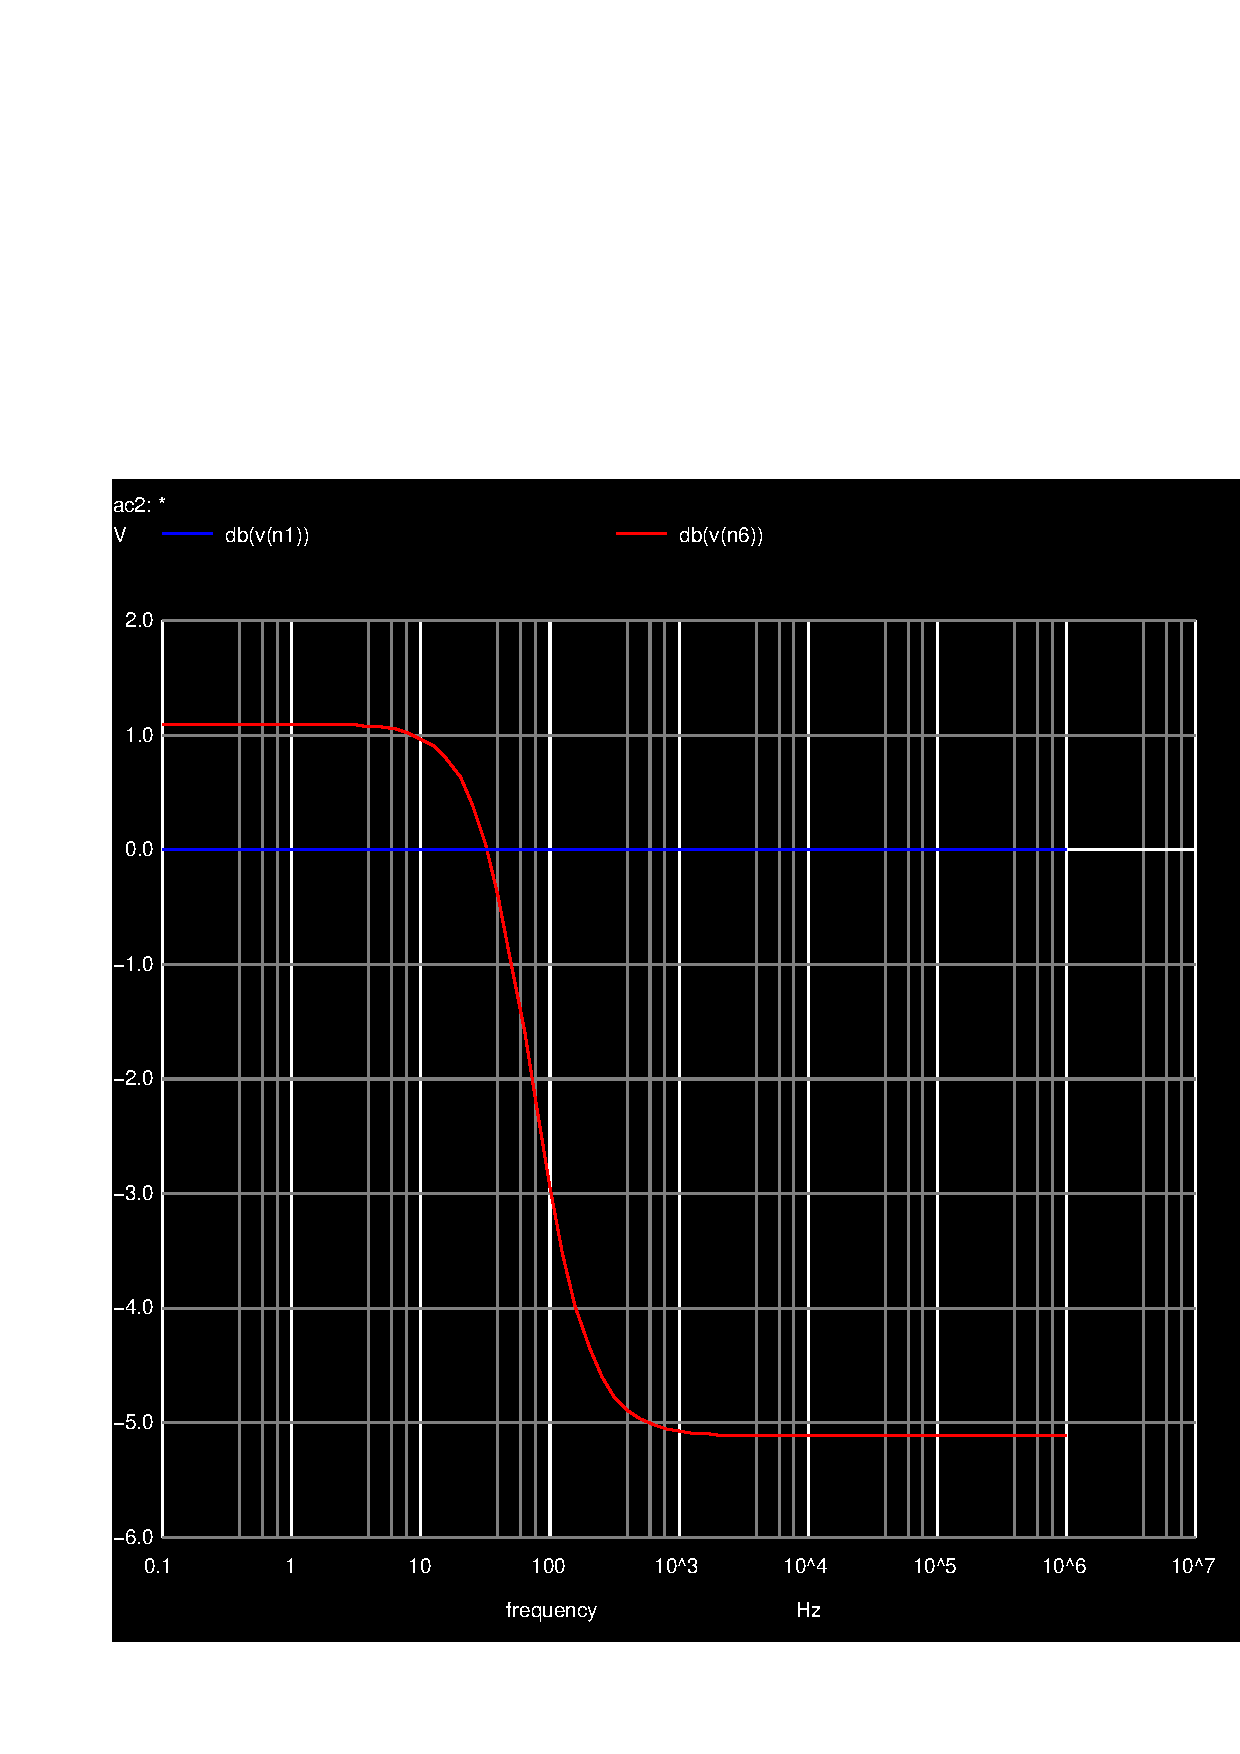
\includegraphics[width=0.7\linewidth]{../sim/fresponse.pdf}
\caption{Frequency Analysis of Question 5.}
\label{fig:fresponse}
\end{figure}
The differences between $v_s(f)$ and $v_6(f)$ are in all ways similar to the reason in question 6 of the theoretical analysis and is described in section 2.6. \par

